\documentclass[]{article}
\usepackage[utf8]{inputenc}

\usepackage{amsmath}
\usepackage{amsfonts}
\usepackage{amssymb}
\usepackage{subcaption}
\usepackage{subfig}

\usepackage{graphicx}
\usepackage{subcaption}
%\usepackage[demo]{graphicx}
%opening
\title{Statistical Data Analysis HW}
\author{Ian Hunt-Isaak}
\date{}
\begin{document}
\maketitle
\section{}
\subsection{Moments of Uniform Distribution based on Definition}

With the uniform distribution:
\begin{equation}
	p_U(x) = \begin{cases}
	\frac{1}{b-a} & a \leq x \leq b\\
	0 & Otherwise
	\end{cases}
\end{equation}
The $0^{th}$ moment:
\begin{align}
M_0 = \int_{-\infty}^{\infty} x^0 p_U(x)dx = \int_{a}^{b} \frac{dx}{b-a} = 1.
\end{align}
The $1^{st}$ moment:
\begin{equation}
M_1 = \int_{a}^{b} \frac{x dx}{b-a} = \frac{1}{2}\frac{b^2-a^2}{b-a} = \frac{1}{2}(a+b) = \mu,
\end{equation}
where $\mu$ is the mean of the distribution. For the higher moments it makes more sense to compute the moments about the mean of the distribution. So for the $2^{nd}$ moment about $\mu$:
\begin{align}
M_2 = \int_{a}^{b} \frac{(x-\mu)^2 dx}{b-a} = \frac{1}{3}\frac{1}{b-a}((b-\mu)^3-(a-\mu)^3) \nonumber \\
= \frac{1}{3}\frac{1}{b-a}((\frac{b-a}{2})^3-(\frac{a-b}{2})^3) \\
= \frac{1}{3}\left(\frac{b-a}{2}\right) \nonumber.
\end{align}
We can see that the 3rd moment will be zero as $(\frac{b-a}{2})^4-(\frac{a-b}{2})^4=0$,

in general the odd moments will be zero. The kth moment will be:
\begin{align}
	M_k = \int_{a}^{b} \frac{(x^k-\mu)^2 dx}{b-a} = \frac{1}{k+1}\frac{1}{b-a}\left((b-\mu)^{k+1}-(a-\mu)^{k+1})\right) \nonumber\\
	= \frac{1}{k+1}\frac{1}{b-a} \left(\left(\frac{b-a}{2}\right)^{k+1}\left(1-(-1)^{k+1}\right)\right) \\
M_k	= \begin{cases}
	0 & \text{k odd}\\
	\frac{1}{k+1}\left(\frac{b-a}{2}\right)^k \nonumber & \text{k even}
	\end{cases}
\end{align}
\subsection{Moments From the Characteristic function}
\begin{align}
\Phi = \int_{-\infty}^{\infty}e^{-i k x}p_U(x)dx = \int_{a}^{b}\frac{1}{b-a}e^{-i k x}dx \nonumber\\
=\left.\frac{i}{k(b-a)}e^{-i k x} \right\vert_a^b\\
= \frac{i}{k(b-a)}\left[e^{-i kb}-e^{-i ka}\right]
\end{align}
To make taking derivatives easier we re-write the exponentials as power series in k.

\begin{align}
\Phi = \frac{i}{k(b-a)} \left[ (1 - i kb +(-i)^2 \frac{k^2b^2}{2!}+ \dots)-\left(1 - i ka +(-i)^2 \frac{k^2a^2}{2!}+ \dots\right)\right] \nonumber\\
= \frac{1}{b-a}\left[(b-a)+(-i) k(b^2-a^2)\frac{1}{2!} + \dots \frac{(-i k)^n}{(n+1)!}(b^{n+1}-a^{n+1})\right]\\
%= \frac{1}{b-a}\left[(b-a)+(-i) k(b-a)\frac{1}{2!} + \dots \frac{(-i k)^n}{(n+1)!}(b-a)^{n+1}\right]
\end{align}
Transforming to be around the mean: ($a\to a-\mu =\frac{a-b}{2}$, $b\to b-\mu =\frac{b-a}{2}$), and taking the nth derivative w.r.t $k$ at $k=0$ then gives us the nth moment:
\begin{align}
(-i)^nM_n = \left.\frac{d^n \Phi}{dk^n}\right\vert_{k=0} = (-i)^n \frac{1}{(n+1)(b-a)}\left[\left(\frac{b-a}{2}\right)^{n+1}- (-1)^{n+1}\left(\frac{b-a}{2}\right)^{n+1}\right] \nonumber\\
M_n = \begin{cases}
0 & \text{n odd} \nonumber\\
\frac{1}{n+1}\left(\frac{b-a}{2}\right)^{n} & \text{n even}
\end{cases}\\
\end{align}
The same result as directly from the definition!.

\section{10m Tall Humans}
I calculate the probability of a 10 m tall human if height were Lorentz distributed as follows:

\begin{align}
y = \frac{10000-a}{L} = \frac{10000-180}{20}\\
p(10000) = \frac{1}{\pi L}\frac{1}{(1+y)^2} = \frac{1}{\pi 20}\frac{1}{(1+820)^2} \approx 6.6\cdot 10^{-8},
\end{align}
or about 7 in a Billion. In contrast if we take Human height to be normally distributed with $\mu=180$ cm and $\sigma=20$, we would find a probability of $~10^{-52532}$, which is effectively zero.

\section{Langevin Equation}
The Langevin Equation (eq \ref{eq:lange}) can be used to describe stochastic processes such as the Motion of a large particle through a sea of smaller particles. 
\begin{align}
\dot{x} = V \nonumber\\
\dot{V} = -\partial_x U -\gamma V(t) + \xi(t)
\label{eq:lange}
\end{align}
This is possible because it takes into account the force from an external potential, a drag term, and a random shock term. The temperature of system can be considered in this system by scaling the random term, $\xi(t)$ by a quantity $V_{\text{thermal}}$. I used the following potential for my simulations of the Langevin equation:

\begin{equation}
	U = -\left[\frac{\sin ((x-2)\pi)}{(x-2)\pi}+\frac{\sin ((x-5)\pi)}{(x-5)\pi}\right].
	\label{eq:potential}
\end{equation}
The potential $U$ and its derivative are both plotted in Figure \ref{fig:potential}. Sampling a linear spacing of initial positions I propagated the simulation particles forward in time for several thousand time steps and recorded and binned their x positions and velocities. The results of this for the Langevin equation with linear damping can be seen in Figure \ref{fig:lange_linear}, and for nonlinear damping in \ref{fig:lange_nonlinear}.

\begin{figure}
	\centering
	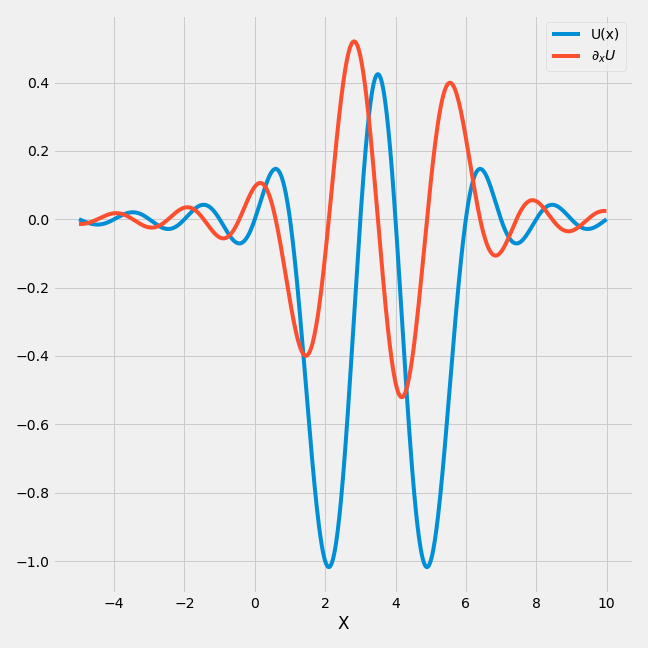
\includegraphics[width=.8\linewidth]{figures/lange_potential.png}
	
	\caption{The potential, and it's derivative, that was used for the Langevin equation simulation. This form was chosen as it gives a double well potential while being easily differentiable. }
	\label{fig:potential}
\end{figure}
\begin{figure}
	\centering
	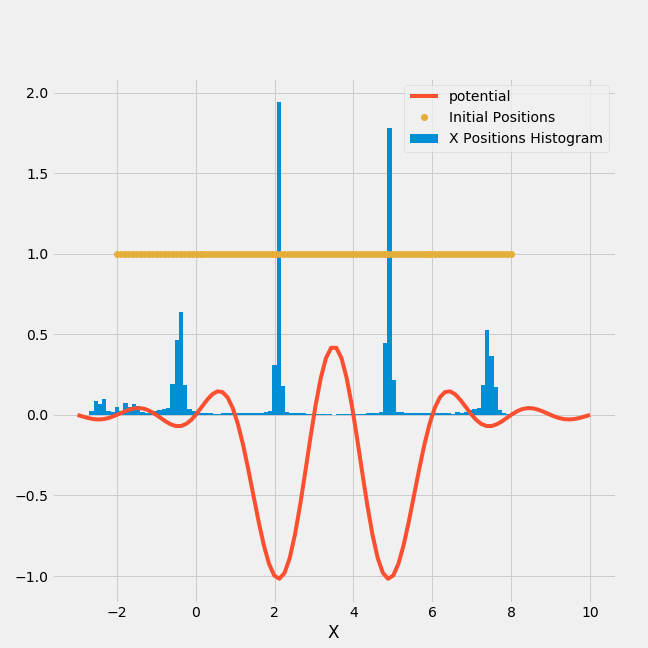
\includegraphics[width=.8\linewidth]{figures/lange_double_well.png}
	
	\caption{Results of my Langevin equation simulation for a double well with potential as defined in Eq. \ref{eq:potential}. As expected we see greater probability density in the regions of the simulation corresponding to the minima of the potential. The blue histogram has been normalized so that the probability density it represents sums to one. }
	\label{fig:lange_linear}
\end{figure}
\begin{figure}
	\centering
	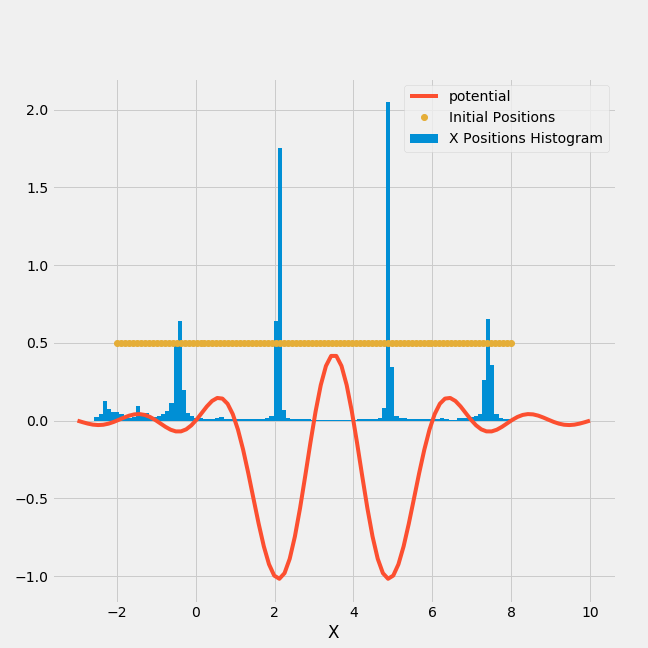
\includegraphics[width=.8\linewidth]{figures/lange_double_well_nonlinear.png}
	
	\caption{Results of my Langevin equation simulation for a double well with potential as defined in Eq. \ref{eq:potential} with a nonlinear damping term $-\gamma V^3$. Compared to the linear damping term the distribution of probability around the wells of the potential is more diffuse. This makes sense as the temperature is the same so similar sized jumps occur, but the particles take longer to relax back to the minimum of the potential. }
	\label{fig:lange_nonlinear}
	\end{figure}
	
\section{Laplace Test Revisited}
I had originally misunderstood the Laplace test and was trying to vary the radius by varying the value of G. This does affect the final radius as it changes the nature of the force, however this is not how the test should be performed. The corrected plot of the Laplace showing the expected linear behavior is below in Figure \ref{fig:laplace} 

\begin{figure}
	\centering
	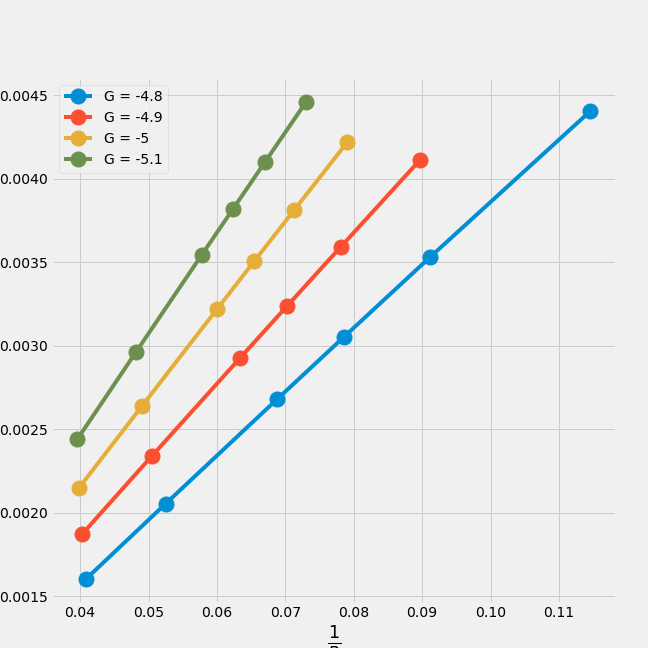
\includegraphics[width=.8\linewidth]{figures/Laplace_test_multG.png}
	
	\caption{Laplace test results from my multiphase Lattice Boltzmann code. This shows the expected linear behavior. The x axis is $\frac{1}{R}$}
	\label{fig:laplace}
\end{figure}
\end{document}